\documentclass[pdftex,twocolumn,10pt,letterpaper]{extarticle}

%%% Set these variables appropriately
%%%
%% Note:  Authors is hardcoded below, this line only used for the PDF info
\newcommand{\AUTHORS}{Sol Boucher, Anuj Kalia, David G. Andersen, and Michael Kaminsky}
\newcommand{\TITLE}{Putting the "Micro" Back in Microservice}
\newcommand{\KEYWORDS}{TODO}
\newcommand{\CONFERENCE}{USENIX ATC '18}
\newcommand{\PAGENUMBERS}{no}       % "yes" or "no"
\newcommand{\COLOR}{yes}
\newcommand{\showComments}{yes}
\newcommand{\comment}[1]{}
\newcommand{\onlyAbstract}{no}

%%%%%%%%%%%%%%%%%%%%%%%%%%%%%%%%%%%%%%%%%%%%%%%%%%%%%%%%%%%%%%%%%%%%%


%%%
%%%  Fonts
%%%
\usepackage[T1]{fontenc}
\usepackage[utf8]{inputenc}
%\usepackage{textcomp}
\usepackage{newtxtext,newtxmath}       % Times/Times-like math symbols
\usepackage{bm}                        % bold math; use \bm{} in captions
\usepackage[scaled=0.92]{helvet}
%\usepackage{courier}
\usepackage[scaled=0.83]{beramono}    % more compact, good for code
%\usepackage{inconsolata}              % another nice alternative to courier


%%%
%%%  Page Setup
%%%
\special{papersize=8.5in,11in}
\setlength{\pdfpagewidth}{8.5in}
\setlength{\pdfpageheight}{11in}

\usepackage{ifthen}
\ifthenelse{\equal{\PAGENUMBERS}{yes}}{%
\usepackage[letterpaper,
            left=1in,right=1in,top=1in,
            footskip=0.5in,bottom=1in,     % Room for page numbers
            columnsep=0.25in
            ]{geometry}
}{%
\usepackage[noheadfoot,left=1in,right=1in,top=1in,
            footskip=0.5in,bottom=1in,
            columnsep=0.25in
	    ]{geometry}
}

%%%
%%%  Captions
%%%
\usepackage[font=bf]{caption}
%%  Space between figure and caption (assuming caption
%%  is below figure)
%\usepackage[font=bf,aboveskip=0pt]{caption} % SPACE
%%  Space between caption and body text of document
%\addtolength{\textfloatsep}{-7pt} % SPACE

%%%
%%%  Section headings
%%%
\usepackage{titlesec}
%\usepackage[compact]{titlesec}              % SPACE
\titlespacing{\paragraph}{0pt}{*1}{*1}      % SPACE
%\titlespacing*{\section}{0pt}{2.5ex plus 1ex minus .2ex}{1.3ex plus .2ex}

%\titleformat{\section}%                     % ACM: caps + period (for 10pt doc)
%  {\bf\large\uppercase}{\thesection.\quad}{0pt}{}

%%% The following should mimic the 9pt ACM sig-alt style headings
%%%
%\titleformat{name=\section}%                 % ACM: caps + period (for 9pt doc)
%  {\bf\LARGE\uppercase}{\thesection.\quad}{0pt}{}
%\titleformat{name=\section,numberless}%      % ACM: for categores, etc.
%  {\bf\LARGE}{}{0pt}{}[\vspace*{-2pt}]
%\titleformat{\subsection}%                   % ACM
%  {\bf\LARGE}{\thesubsection\quad}{0pt}{}
%\titleformat{\subsubsection}%                % ACM
%  {\it\Large}{\thesubsubsection\quad}{0pt}{}

%%%
%%%  Lists
%%%
\usepackage{enumitem}
\setlist{itemsep=0pt,parsep=0pt,topsep=0pt}             % more compact lists

%%%
%%%  Header / Footer
%%%
\usepackage{fancyhdr}
\renewcommand{\headrulewidth}{0pt}

\ifthenelse{\equal{\PAGENUMBERS}{yes}}{%
  \pagestyle{plain}
}{%
  \pagestyle{empty}
}

%%%
%%%  Bibliography
%%%
\usepackage[numbers]{natbib}

%%%
%%%  Footnotes / Endnotes
%%%
\interfootnotelinepenalty=10000  % Split footnotes are annoying

% If you want endnodes, uncomment:
%\usepackage{endnotes}
%\usepackage{drafthead}
%\let\footnote=\endnote

%%%
%%%  Tables
%%%
\usepackage{booktabs}
\usepackage{color}
\usepackage{colortbl}
\usepackage{float}                           % Must appear before hyperref to
                                             % avoid weird PDF compile issues
\usepackage{multirow}

%%%
%%% Special commands
%%%
\usepackage[binary-units=true]{siunitx}
\newcommand{\ns}[1]{\SI{#1}{\nano\second}}
\newcommand{\us}[1]{\SI{#1}{\micro\second}}
\newcommand{\ms}[1]{\SI{#1}{\milli\second}}
\newcommand{\byte}[1]{\SI{#1}{\byte}}
\newcommand{\kbyte}[1]{\SI{#1}{\kilo\byte}}
\newcommand{\mbyte}[1]{\SI{#1}{\mega\byte}}
\newcommand{\gbyte}[1]{\SI{#1}{\giga\byte}}
\newcommand{\Gbps}[1]{\SI{#1}{Gbps}}
\newcommand{\GHz}[1]{\SI{#1}{GHz}}
\newcommand{\GbE}[1]{\SI{#1}{GbE}}
\newcommand{\GBps}[1]{\SI{#1}{GBps}}
\newcommand{\Mrps}[1]{\SI{#1}{Mrps}}

%%%
%%%  PDF setup
%%%
\ifthenelse{\equal{\COLOR}{yes}}{%
  \usepackage[colorlinks,citecolor=blue]{hyperref}%         % for online version
}{%
  \usepackage[pdfborder={0 0 0}]{hyperref}%  % for paper (B&W) version
}
\usepackage{url}

\hypersetup{%
pdfauthor = {\AUTHORS},
pdftitle = {\TITLE},
pdfsubject = {\CONFERENCE},
pdfkeywords = {\KEYWORDS},
bookmarksopen = {true}
}

% Anonymize figure inclusion
% Requires pdfTeX version 1.40.17
%\pdftrailerid{} %Remove ID
%\pdfsuppressptexinfo15 %Suppress PTEX.Fullbanner and info of imported PDFs

% Uncomment next line if your printer outputs black
% boxes instead of drop shadows; older PDF interpreters
% in printers can't handle those PDF 1.5 features
%\pdfminorversion=3
%\pdfobjcompresslevel=2


%%
%% Figure placeholder macros
%%

\definecolor{placeholderbg}{rgb}{0.85,0.85,0.85}
\newcommand{\placeholder}[1]{%
\fcolorbox{black}{placeholderbg}{\parbox[top][1.5in][c]{0.95\columnwidth}{#1}}}


%%%
%%%  Misc
%%%
\usepackage[pdftex]{graphicx}
\usepackage{soul}
% this allows \st and friends to work with citations
\soulregister\cite7
\soulregister\ref7
\soulregister\pageref7

\makeatletter
\newlength{\secaskip}
\newlength{\secbskip}
\let\@section\section
\renewcommand{\section}{\@ifstar{\section@star}{\section@nostar}}
\newcommand{\section@nostar}[1]{\vspace{\secbskip}\@section{#1}\vspace{\secaskip}}
\newcommand{\section@star}[1]{\vspace{\secbskip}\@section*{#1}\vspace{\secaskip}}
\let\@subsection\subsection
\renewcommand{\subsection}{\@ifstar{\subsection@star}{\subsection@nostar}}
\newcommand{\subsection@nostar}[1]{\vspace{\secbskip}\@subsection{#1}\vspace{\secaskip}}
\newcommand{\subsection@star}[1]{\vspace{\secbskip}\@subsection*{#1}\vspace{\secaskip}}
\newlength{\parsecskip}
\let\@paragraph\paragraph
\renewcommand{\paragraph}[1]{\vspace{\parsecskip}\@paragraph{#1}}
\makeatother

\setlength{\secaskip}{-6pt}
\setlength{\secbskip}{-12pt}
\setlength{\parsecskip}{-4pt}

%\setlength{\parindent}{0pt}
\setlength{\parskip}{0pt}

\setlength{\abovecaptionskip}{6pt}
\setlength{\belowcaptionskip}{-12pt}

%\clubpenalty=10000  % Don't allow orphans
%\widowpenalty=10000 % Don't allow widows

%%%
%%%  To appear/appeared in text on title page
%%%
\usepackage[absolute]{textpos}
\newcommand{\ToAppear}{%
\begin{textblock*}{\textwidth}(0.95in,0.4in)
\begin{flushright}
    %\noindent{\fbox{\textsf{Under submission---please do not redistribute.}}}
    %  --OR--
    \noindent{\small To appear in \textit{Proceedings of the XYZ}\\
    \noindent{\small \textit{Conference (XYZ'08)}, City, State, Month 2008}}
    %  --OR--
    %\noindent{\small In \textit{Proceedings of the XYZ}\\
    %\noindent{\small \textit{Conference (XYZ'08)}, City, State, Month 2008}}
\end{flushright}
\end{textblock*}
}

%%%
%%%  Sample ACM Copyright Block
%%%
\newfloat{acmcr}{b}{acmcr}
\newcommand{\AcmCopyright}{%
\begin{acmcr}
\parbox[b]{20pc}{%
\footnotesize
Permission to make digital or hard copies of all or part of this work
for personal or classroom use is granted without fee provided that
copies are not made or distributed for profit or commercial advantage
and that copies bear this notice and the full citation on the first
page.  To copy otherwise, to republish, to post on servers or to
redistribute to lists, requires prior specific permission and/or a fee.

{\em Conference}, Month Date--Date, Year, Location\\
Copyright 200X ACM X-XXXXX-XX-X/XX/XX ...\$5.00}
\end{acmcr}}

%%%
%%%  Comments
%%%
\newcommand{\note}[2]{
    \ifthenelse{\equal{\showComments}{yes}}{\textcolor{#1}{#2}}{}
}

% Change these to your own initials as you like...
\newcommand{\dga}[1]{\note{blue}{DGA: #1}}
\newcommand{\mk}[1]{\note{red}{MK: #1}}
\newcommand{\solb}[1]{\note{green}{SOLB: #1}}
\newcommand{\ak}[1]{\note{magenta}{AK: #1}}

\date{}
\title{\vspace{-1.6em}\textbf{Putting the ``Micro'' Back in Microservice}}
\author{{\large Sol Boucher*, Anuj Kalia*, David G. Andersen*, and Michael Kaminsky$^\dagger$}\\
{\em * Carnegie Mellon University \; $^\dagger$ Intel Labs}}

% This needs to be the last thing before \begin{document}
\usepackage{microtype}  % SPACE

%%%%%%%%%%%%%%%%%%%%  START DOCUMENT  %%%%%%%%%%%%%%%%%%%%%%%%
\begin{document}

\maketitle

\ifthenelse{\equal{\PAGENUMBERS}{yes}}{%
  \thispagestyle{fancy}
}{%
  \thispagestyle{empty}
}

%\AcmCopyright
%\ToAppear

We introduce novel programming abstractions for isolation of both time and memory.
They operate at finer granularity than traditional primitives, supporting preemption
at sub-millisecond timescales and tasks defined at the level of a function call.
This resolution enables new functionality for application programmers, including
users of unmanaged systems programming languages, all without requiring changes to
the existing systems stack.  Despite being concurrency abstractions, they employ
synchronous invocation to allow application programmers to make their own scheduling
decisions.  However, we found that they compose naturally with existing concurrency
abstractions centered around asynchronous background work, such as threads and
futures.  We demonstrated how such composition can enable asynchronous cancellation
of
threads and the implementation of preemptive thread libraries in userland, both
regarded for decades as challenging problems.

\ifthenelse{\equal{\onlyAbstract}{no}}{%
\section{Introduction}
\label{sec:intro}

As the scope and scale of Internet services continues to grow, system designers
have sought platforms that simplify scaling and deployment.
Services that outgrew self-hosted servers moved to datacenter racks, then
eventually to virtualized cloud hosting environments.
However, this model only partially delivered two related benefits:
\begin{enumerate}
\item Pay for only what you use at very fine granularity
\item Scale up rapidly on demand
\end{enumerate}

\noindent
The VM approach suffered from relatively coarse granularity:  Its atomic compute unit
of machines were billed at a minimum of minutes to months.  Relatively long startup
times often required system designers to keep some spare capacity online to handle
load spikes.

These shortcomings led cloud providers to introduce a new model, known as
serverless computing, in which the customer provides \textit{only} their code,
without having to configure its environment.   Such ``function as a service''
(FaaS) platforms are now available as AWS Lambda~\cite{www-amazon-lambda}, Google
Cloud Functions~\cite{www-google-cf}, Azure Functions~\cite{www-microsoft-af}, and
Apache OpenWhisk~\cite{www-apache-openwhisk}.  These platforms provide a model in
which: (1)  user code is invoked whenever some event occurs (e.g., an HTTP
API request), runs to completion, and nominally stops running (and being
billed) after it completes; and (2)  there is no state preserved between
separate invocations of the user code.  Property (2) enables easy auto-scaling
of the function as load changes.

Because these services execute within a cloud provider's
infrastructure, they benefit from low-latency access to other cloud
services.  In fact, acting as an access-control proxy is a recurring microservice
pattern:\@ receive an API request from a user, validate it, then access
a backend storage service (e.g., S3) using the service's credentials.

In this paper, we explore a design intended to reduce the tension between two of
the desiderata for cloud functions:\@ low latency invocation and low cost.  Contemporary
invocation techniques exhibit high latency with a
large tail; this is
unsuitable for many modern distributed systems which involve
high-fanout communication, sometimes performing thousands of
lookups to handle each user request.  Because user-visible response time often
depends on the tail latency of the slowest chain of dependent
responses~\cite{Dean:cacm2013}, shrinking the tail is crucial~\cite{Jalaparti:sigcomm2013,
Xu:nsdi2013,Li:socc2014,Jeon:asplos2016}.

Thus we seek to reduce the invocation latency and improve predictability, a
goal supported by the impressively low network latencies available in modern
datacenters. For example, it now takes $<20\mu{}s$ to perform an RPC between two
machines in
Microsoft Azure's virtual machines~\cite{Firestone:nsdi2018}. We believe,
however, that fully leveraging this improving network performance will require
reducing microservices' invocation latencies to the point where the network is
once again the bottleneck.

We further hypothesize---admittedly without much proof for this chicken-and-egg
scenario---that substantially reducing both the latency and cost of running
intermittently-used services will enable new classes and scales of applications
for cloud functions, and in the remainder of this paper, present a design that
achieves this.  As Lampson noted, there is power in making systems 
``fast rather than general or powerful''~\cite{Lampson1983}, because fast
building blocks can be used more widely.

Of course, a microservice is only as fast as the slowest service it relies on;
however, recall that many such services are offered in the same clouds and
datacenters as serverless platforms. Decreasing network latencies will push
these services to respond faster as well, and new stable storage
technologies such as 3D XPoint (projected to offer sub-microsecond reads and
writes) will further accelerate this trend by offering lower-latency storage.

In this paper, we propose a restructuring of the serverless model centered around
low-latency: \textit{lightweight microservices} run in \textit{shared processes}
and are isolated primarily with language-based \textit{compile-time guarantees} and
\textit{fine-grained preemption}.

%% \subsection{Not yet rewritten}

%% At the time of writing, AWS Lambda, Azure Functions, and Google Cloud Functions
%% cap instance execution time to 5--10 minutes.

%% \solb{AK: I see you touched this recently.  Do you still want to see us say it (and
%% where)?  I currently mention penultimate section of Motivation and related work that
%% providers presently impose a limit, without actually saying what it is.}
%% \mk{This subsection seems out of place.}

\section{Building Blocks}
\label{sec:motive}

\begin{table}
\begin{center}
\small
\begin{tabular}{lrrr}
   & \multicolumn{2}{c}{\textbf{Latency (µs)}} & \textbf{Throughput} \\
  \textbf{Isolation method} & Median & 99\% & \textbf{(invocations/sec)} \\
\midrule
Process-based & 8.7 & 27.3 & 288,625 \\
Language-based & 1.2 & 2.0 & 5,418,889 \\
\end{tabular}
\caption{Performance of isolation methods}
\label{tab:isolation_methods}
\end{center}
\end{table}

Our decision to use language-based isolation is based on two experimental
results that we discuss below. First, process-level isolation is too slow for
microsecond-scale remote functions. Second, high-precision timers on commodity
CPUs allow premption at microsecond scale. The experiments in this paper were
conducted on an Intel Xeon E5-2683 v4 CPU (16 cores, 2.1~GHz), running
Linux 4.13.0.

\subsection{Process-level isolation is too slow}
We run the following experiment to evaluate the overhead of different isolation
techniques. We use 14 \emph{worker} CPU cores to run microservices. Another core runs
runs a \emph{host} process that initiates microservice execution on the workers.
The host schedules up to 14 microservices at a time (i.e., one
per worker core), choosing from a pool of 5,000 microservices. It uses one of two
methods to run microservices:

\begin{enumerate}
\item \textbf{Process-based isolation:} Each microservice is a separate process.
At any time, most microservice processes are blocked on an IPC
call. The host runs a microservice by waking up its process using IPC. We use
UDP datagrams for IPC; other IPC methods perform similarly~XXXcite.
\item \textbf{Language-based isolation:} Each worker core runs a single-threaded
\emph{worker process} that is used to run different microservices, one at a time.
In this approach, shown in Figure~\ref{fig:sysdesign}, a worker process runs a
microservice by calling its registered
function; we assume that the microservice function can be isolated from the
worker process with language-based isolation techniques that we discuss in
Section~\ref{sec:isolation}. The host schedules microservices on worker processes by
sending them
requests on a shared memory queue. Worker processes poll this queue to receive
new requests.
\end{enumerate}

\begin{figure}
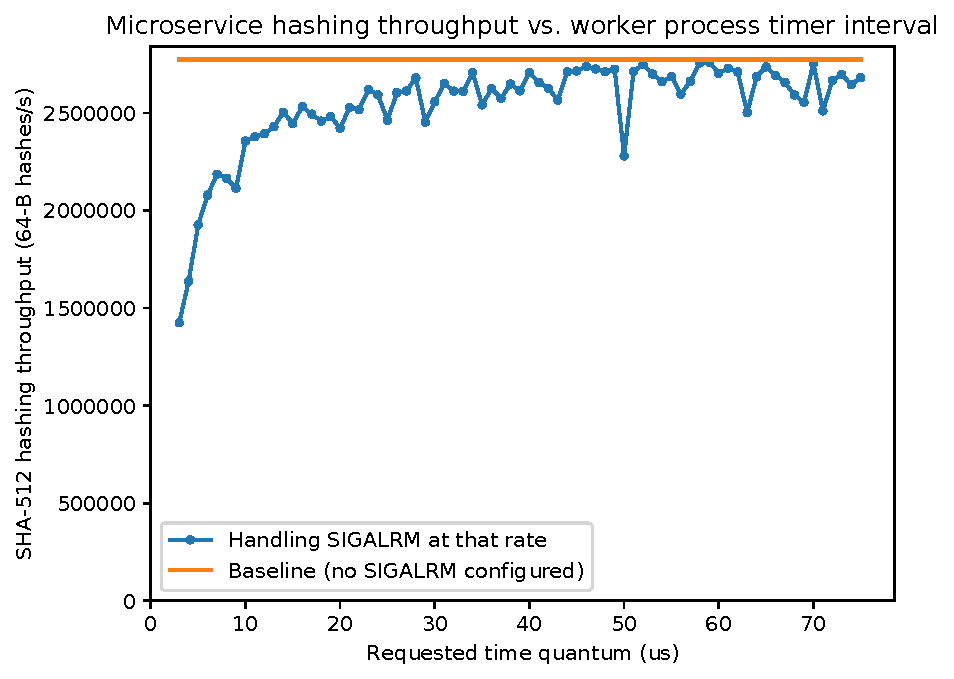
\includegraphics[width=\columnwidth]{figs/system}
\caption{Design of the language-based isolation approach.  The host process forwards
requests over a shared-memory queue to a number of worker processes, each of which
runs one user-supplied microservice at a time.}
\label{fig:sysdesign}
\end{figure}

Table~\ref{tab:isolation_methods} shows the latency and throughput achieved
by the two methods. For latency, we measure the time between when the host
process dispatches a request to a microservice and when the service begins
useful work on a worker core. We find that the process-based isolation approach
takes 9\textmu{}s and achieves only 300,000 microservice invocations per
second. In contrast, language-based isolation achieves 1.2\textmu{}s (with a tail
of just 2.0\textmu{}s) and over 5 million invocations per second\footnote{We also
observe that, with trivial microservices, there is a difference in memory
footprint:\ for 5,000 resident microservices, the system memory usage rises by about
2 GiB for the process-based approach, versus just 1.3 for the language-based one.  Of
course, these numbers will substantially rise for larger programs, but we expect the
gap to widen as various microservices include the same libraries.}

A 9\textmu{}s delay in microservice invocation is a substantial fraction of our
20\textmu{}s RPC latency; \mk{What is ``our''?} the fraction is likely to increase with
improvements in network latency. We therefore conclude that process-based
isolation is too slow for microsecond-scale scheduling; furthermore, invocation
throughput is also limited by IPC overhead.

\subsection{Intra-process preemption is fast}
With language-based isolation, we run user-provided microservice functions
directly in worker processes. To prevent rogue functions from endlessly blocking
other microservices, we must premept or terminate functions that run for too
long (e.g., longer than 100\textmu{}s).  This
preemption interval is orders of magnitude faster than typical operating
system preemption intervals ($\approx$5ms).
\mk{Can we add a citation here?}

Fortunately, we found that high-precision event timers (HPETs) on modern CPUs
are sufficient for this task. We measure the granularity and reliability of
these timers as follows: We run one thread that installs a timer that fires
periodically at configurable intervals of $T$\textmu{}s. We install a signal
handler that is called on each timer interrupt. Ideally, the signal handler
would be called for the $i^{th}$ time at $T + i$\textmu{}s; we measure the
average difference over 100 iterations between $T + i$ and the actual time
when the signal handler runs for the $i^{th}$ time. We find that the variance
is smaller than 0.3\textmu{}s for $T > Y$\textmu{}s. This shows that
intra-process premeption is fast and reliable enough for our needs.
\mk{This is a bit confusing.}

\section{Providing Isolation}
\label{sec:isolation}

Consolidating multiple users' jobs into a single process requires
addressing security and isolation. We aim to do this in a way that does not
compromise our ambitious performance goals.

Our guiding philosophy for doing so is ``Language-based isolation with defense in depth.''
We draw inspiration from two recently-published systems whose own demanding
performance requirements drove them to perform similar coalescing of traditionally
independent components:  NetBricks~\cite{Panda2016} is a network functions runtime
for providing programmable network capabilities; it is unique among this class of
systems for running network functions from different vendors in-process rather than in VMs.
Tock~\cite{Levy2017} is an embedded operating system that provides (in addition to a
more traditional process model) a type of lightweight application known as a capsule
that is embedded within the kernel and communicates with it using simple function
calls.  As their primary line of defense against untrusted code, both systems
leverage Rust~\cite{www-rustlang}, a new type-safe systems programming language.


Rust is a strongly-typed, compiled language that uses a lightweight runtime
similar to C.  Unlike many other modern systems languages, Rust is an
attractive choice when predictable performance is critical due to its
lack of a garbage collector.  Still, it manages to provide strong memory safety
guarantees by focusing on ``zero-cost abstractions'' (i.e., those that can be
compiled down to code whose safety is assured without runtime checks).  In
particular, safe Rust code is guaranteed to be free of null or dangling pointer
dereferences, invalid variable values (e.g., casts are checked and unions are
tagged), reads from uninitialized memory, mutations of non-\texttt{mut} data (roughly
the equivalent of C's \texttt{const}), and data races, among other
misbehaviours~\cite{www-rustlang-ub}.

We require each microservice to be written in Rust, which gives us many aspects of
the isolation we need:  It is difficult for microservices to crash the worker process,
since most segmentation faults are prevented, and runtime errors such as integer
overflow generate Rust panics that we can catch.  Microservices cannot get references
to data that does not belong to them thanks to the variable and pointer initialization
rules.

Given our performance goals, there is a crucial isolation aspect that
Rust does not provide: there is nothing to stop users from monopolizing the CPU\@.
Our system, however, must be preemptive. We are unaware of existing preemption
techniques that work at microsecond scales. Note that coroutine-like
cooperative multitasking approaches (such as lightweight threads in
Go~\cite{www-golang} and Erlang~\cite{www-erlang}) are not preemptive, so they
do not work for us. We discuss our solution to this in the following section;
it depends on installing a \texttt{SIGALRM} handler and ensuring that trusted
code within the process handles the signal.

Our defense-in-depth comes from using lightweight operating-system protections
to block access to certain system calls, as well as the proposed mechanisms
in Section~\ref{sec:future}.  Some system calls must be blocked to have any
defense at all; 
otherwise, the microservice could disable the \texttt{SIGALRM}-based preemption
(e.g., \texttt{signal()}), create kernel threads (e.g., \texttt{fork()}),
create competition between threads (e.g., \texttt{nice()}), or even terminate
the entire worker (e.g., \texttt{exit()}). Finally, user functions should not
have unmonitored file system access.

We block access to system calls using the \texttt{seccomp()} system call~\cite{seccomp-manpage}
to have each worker process lock itself down during initialization,
thereby limiting the process to a
whitelisted set of system calls.  Prior to lockdown, the worker
process installs its \texttt{SIGALRM} handler for preemption, and
a  \texttt{SIGSYS} handler and tear down the running microservice if it is
ever received.


\section{Providing Preemption}
\label{sec:preemption}

% \solb{I was thinking of basing the conclusion off this; maybe it should just
% \textit{be} there?}
% 
% \solb{Is it weird to have the following paragraph after we discuss isolation and
% preemption?  I can't think of where else it would go.}
% 
% Our system comprises (1) a central dispatch process that manages the compute node,
% receiving requests and assigning them to (2) a number of worker processes (one per
% dedicated compute core) via a shared memory region.  Each worker process runs a
% tight loop that polls on a ready bit in shared memory; once it finds work to be done,
% it sets itself up to catch any runtime panic and jumps into user code.  The worker
% process receives frequent \texttt{SIGALRM}s to ensure it never loses control of its
% CPU:\ in the associated handler, it checks how for long the current job has been
% running and ends any that has gone over budget.  The rest of this section covers the
% trust model and the preemption scheme.

% <snip>

%\paragraph{Preemption scheme}

The system must be able to detect and recover from microservices that, whether
maliciously or negligently, attempt to run for longer than permitted.  The two parts
of this problem are (1) regaining control of the CPU and (2) aborting and cleaning up
after the user code.

As proposed in Section~\ref{sec:motive}, regaining control of the CPU happens when a
signal (\texttt{SIGALRM}) from the kernel transfers control to the worker process's
handler.  The handler then checks how long the current microservice has been running
and decides whether it should be killed.  (We register the handler using the
\texttt{SA\_RESTART} flag to \texttt{sigaction()} so that any interrupted blocking
syscalls are restarted transparently.)  However, there remain three important
questions:

\paragraph{For how long should each microservice be allowed to run?}
%Consider a well-utilized but not overloaded compute node in which a user task
%is executing on each available core, but there is no backlog behind which an incoming task must wait.
Assume, as in Section~\ref{sec:motive}, that each core executes one user task at a
time and that all microservice
functions are pre-compiled and resident (warm invocation).
%The impact of microservice runtime on tail latency in 
%(This being preliminary work, any discussion of the cluster-level
%scheduling responsible for these theoretical conditions are outside the scope of
%this paper.)
%Furthermore, we'll assume an incoming microservice that is warm on each
%worker thread.
We define $L$ to be the desired invocation latency, $B$ to be the
runtime budget allotted to each microservice, and $r_c$ to be the remaining runtime
of the microservice on CPU $c$.  Thus, in the worst case (where all tasks are
executing for their entire allotted time) the probability that the incoming
microservice will have somewhere to run in time to meet the invocation
latency SLO is given by:
\begin{equation}
p(r_\textrm{min} \le L) = \sum\limits_{c \in C} p(r_c \le L) = \big| C \big| \frac{L}{B}
\end{equation}
Given the 14 cores in our setup and imagining we want to keep the 99\% tail,
$p(r_\textrm{min} \le L) = 0.99$, to an $L$ of 8~$\mu{}s$, we need to kill tasks
running for more than 113~$\mu{}s$.

\paragraph{How often should the handler execute (the \emph{quantum})?}
We showed at the end of Section~\ref{sec:motive} that microsecond-scale preemption is
\textit{achievable}, but can it be done \textit{efficiently}?  To find out, we wrote
a microservice that measures the throughput of computing SHA-512 hashes over 64 B of
data at a time.  We then subjected its worker process to \texttt{SIGALRM}s, varying
the quantum and observing the resulting hashing throughput.
Figure~\ref{fig:hashtput} illustrates that by a quantum of about 20 $\mu{}s$,
throughput had reached 90\% of baseline.  Considering this an acceptable performance
degradation, we adopt this quantum and prescribe a runtime budget of 93 $\mu{}s$ so
that we can always kill over-budget microservices in time to avoid violating our tail
latency SLO.

\begin{figure}
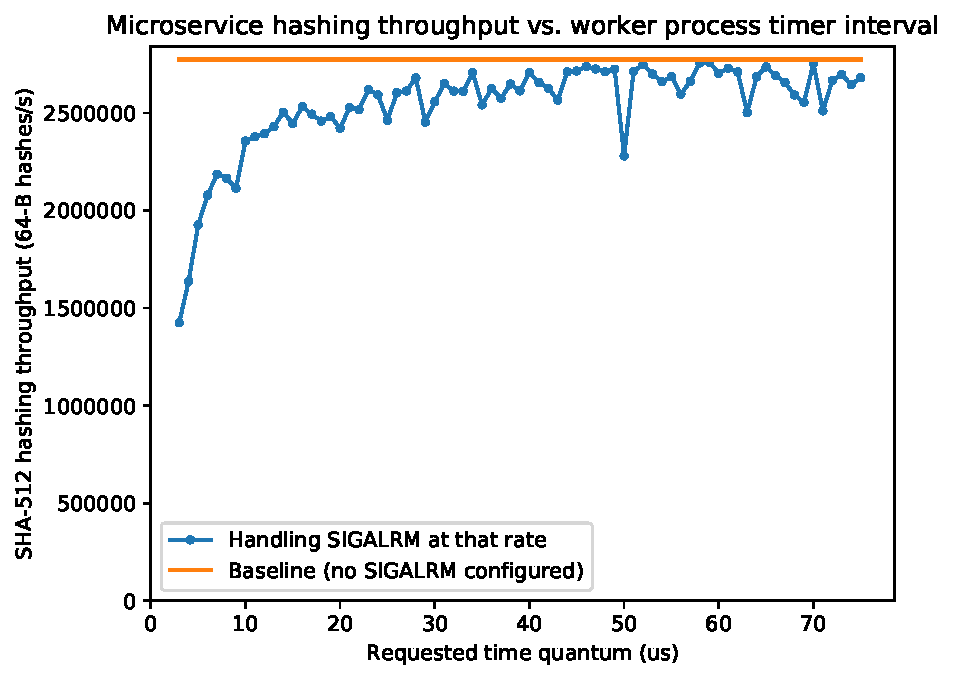
\includegraphics[width=\columnwidth]{figs/2018-02-02-evaluation_quantum-hasher_throughput-throughput}
\caption{Effect of \texttt{SIGALRM} quantum on SHA hashing throughput}
\label{fig:hashtput}
\end{figure}

\paragraph{How do we clean up a terminated microservice?}
We now discuss the mechanism for aborting
and cleanup.  POSIX signal handlers receive as an argument a pointer to their
\textit{context}, a snapshot of the process's PCB (process control block) at the
moment before it received the signal.  When the handler returns, the system will
transfer control back to the point described by the context, so a naïve way for our
worker processes to regain control would be to reset its GPRs (general-purpose
registers) to values recorded just before the worker's tight scheduling loop.
This approach, however, would not release the microservice's state or memory
allocations back to the worker.

One of the few heavyweight components of the Rust runtime is panic handling,
reminiscent of C++'s exception handling.  The compiler inserts landing pads into each
function that call the destructors for the variables in its stack frame, and if the
program ever panics,
the standard library unwinds the stack, jumping to each landing pad in turn.  We
co-opt this functionality by having the \texttt{SIGALRM} handler set its context
to describe executing a function that raises an explicit panic in a fake stack frame
just above the real top of the stack.

Section~\ref{sec:future} discusses several limitations and security
ramifications of this approach.

However, there remain three important
questions:

\paragraph{For how long should each microservice be allowed to run?}
%Consider a well-utilized but not overloaded compute node in which a user task
%is executing on each available core, but there is no backlog behind which an incoming task must wait.
Assume that each core executes one user task at a
time and that all microservice
functions are pre-compiled and resident (warm invocation).
%The impact of microservice runtime on tail latency in 
%(This being preliminary work, any discussion of the cluster-level
%scheduling responsible for these theoretical conditions are outside the scope of
%this paper.)
%Furthermore, we'll assume an incoming microservice that is warm on each
%worker thread.
We define $L$ to be the desired warm invocation latency, $B$ to be the
runtime budget allotted to each microservice, and $r_c$ to be the remaining runtime
of the microservice on CPU $c$.  Thus, in the worst case (where all tasks are
executing for their entire allotted time) the probability that the incoming
microservice will have somewhere to run in time to meet the invocation
latency SLO is given by:
\vspace{-10pt}
\begin{equation}
p(r_\textrm{min} \le L) = \sum\limits_{c \in C} p(r_c \le L) = \big| C \big| \frac{L}{B}
\vspace{-10pt}
\end{equation}
Given the 14 cores in our setup and imagining we want to keep the 99\% tail,
$p(r_\textrm{min} \le L) = 0.99$, to an $L$ of 8~$\mu{}s$, we need to kill tasks
running for more than B = 113~$\mu{}s$.

\paragraph{How often should the handler execute (the \emph{quantum})?}
We showed in Section~\ref{sec:motive} that microsecond-scale preemption is
\textit{achievable}, but can it be done \textit{efficiently}?  To find out, we wrote
a microservice that measures the throughput of computing SHA-512 hashes over 64 B of
data at a time.  We then subjected its worker process to \texttt{SIGALRM}s, varying
the quantum and observing the resulting hashing throughput.
Figure~\ref{fig:hashtput} illustrates that by a quantum of about \us{20}, throughput
had reached around 90\% of baseline.  Considering this performance degradation,
acceptable we adopt this quantum and prescribe a runtime budget of 113 - 20 = \us{93}
so that we can kill over-budget microservices in time to avoid violating our tail
latency SLO.

\begin{figure}
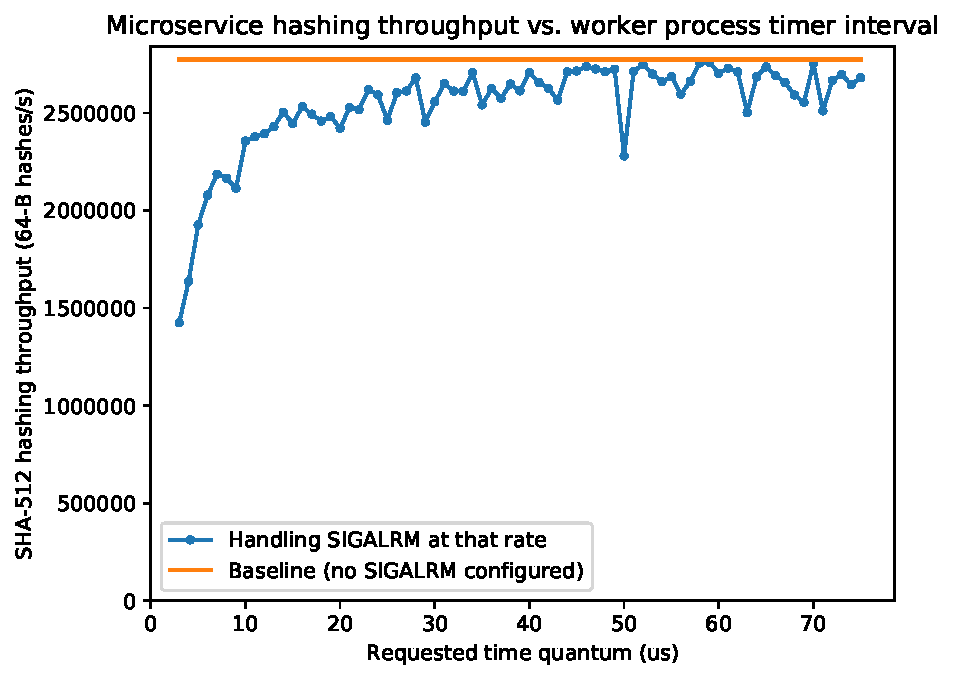
\includegraphics[width=\columnwidth]{figs/2018-02-02-evaluation_quantum-hasher_throughput-throughput}
\caption{Effect of \texttt{SIGALRM} quantum on hashing tput.}
\label{fig:hashtput}
\end{figure}

\paragraph{How do we clean up a terminated microservice?}
We now discuss our mechanism for aborting and cleaning up after a microservice
exceeds its runtime budget.  POSIX signal handlers receive as an argument a pointer to their
\textit{context}, a snapshot of the process's PCB (process control block) at the
moment before it received the signal.  When the handler returns, the system will
transfer control back to the point described by the context, so a naïve way for our
worker processes to regain control would be to reset its GPRs (general-purpose
registers) to values recorded just before the worker's tight scheduling loop.
This approach, however, would not release the microservice's state or memory
allocations back to the worker.

One of the few heavyweight components of the Rust runtime is panic handling,
reminiscent of C++'s exception handling.  The compiler inserts landing pads into each
function that call the destructors for the variables in its stack frame:\@ if the
program ever panics, the standard library uses these to unwind the stack.  We co-opt
this functionality by having the \texttt{SIGALRM} handler set its context to raise an
explicit panic in a fake stack frame just above the real top of the stack.

Section~\ref{sec:future} discusses the limitations and security ramifications of
this approach.


\section{Deployment}
\label{sec:deploy}

We now describe our microservices in the broader context of our full proposed
serverless system.  We clarify their lifecycle, interactions with the compute nodes,
and the trust model for the cloud provider.

Users submit their microservices in the form of Rust source code, allowing the
serverless operator to pass the \texttt{-Funsafe-code} compilation flag to reject
any \texttt{unsafe} code.  This process need not occur on the compute
nodes, provided the deployment server tasked with compilation runs the same version
of the Rust compiler\footnote{This restriction exists because, as of the latest
release (1.23.0) of the compiler, Rust does not have a stable ABI.}.  The operator
needs to trust the compiler, standard library, and any libraries against which it
will permit the microservice to link (since they might contain \texttt{unsafe} code),
but importantly need not worry about the microservice itself.

We believe that many users would find it acceptable to be presented with a specific
list of permitted dependencies.  But how big a list could the provider hope to offer
at the time of launching the service?  It bears noting that libraries including only
safe Rust code could be whitelisted without review.  To approximate how big such a
list would be given the current Rust ecosystem, we turn to a 2017
study~\cite{www-cratesio-unsafe} by the Tock authors that found just under half of
the Rust package manager's top 1000 most-downloaded libraries to be free of
\texttt{unsafe} code.  They caution that many of those packages have unsafe
dependencies, but we suspect that reviewing a relatively small number of popular
libraries would open up the majority of the most popular packages.

If the application compiles (is proven memory-safe) and links (depends only on
trusted libraries) successfully, the deployment server produces a shared object file,
which the provider then distributes to each compute node on which it might run.
Then, in order to ensure that invokers will experience the warm-start latencies
discussed in Section~\ref{sec:motive}, those nodes' host processes should instruct
one or more of their workers to preload the dynamic library.  If the provider
experiences too many active microservices for its available resources, it can
unload some libraries; on their next invocation, they will experience higher
(cold start) invocation latencies since we need to synchronously load the dynamic
library.  In our measurements, the overhead of this operation is about 100\textmu{}s.

\section{Future work}

\solb{This isn't exactly a future work section, is it...?}

Like \textit{Shinjuku} and \textit{RT} before us, we have arrived at a preemptive
thread library; however, we have done so by building parallelism on top of
not the other way around.  Because of this, we have a more flexible abstraction, and
we intend to continue applying it to other problems.

\solb{Mention other use cases, such as the continuation-memoizing RPC server?}

But we have also diverged from \textit{Shinjuku} and \textit{RT}
in another way:\@ unlike these systems, we make each thread responsible for
its own preemption rather than serving preemption signals from a shared watchdog
thread.  This decision was informed by back-of-the-envelope calculations based on
Shinjuku's comparison of the end-to-end latency of bare-metal interprocessor
interrupts (IPIs) versus Linux signals.

While Shinjuku reports that IPIs take an average of only 1,993 cycles, compared to
4,950 for signals (roughly 1:2.5), their sender/receiver breakdown of the latter
number suggests significant latency savings by avoiding cross-core signaling:
First, 343 of those cycles (6.9\%) are spent propagating the signal between the two
cores; we expect this delay to be nearly absent for a timer interrupt originating at
its destination core's own local interrupt controller.  Second, 2,084 cycles (42\%)
are incurred by the sending core; assuming the interrupt controller supports
periodic timer interrupts at the necessary frequency, this cost does not need to be
paid between each interrupt, suggesting measurable savings here too.  Although
our prototype is not yet optimized to this extent, we expect it is possible for a
system built on intra-thread Linux signals to achieve an average preemption latency
within 2x that of Shinjuku's custom operating system.  It is our hope that further
optimization of our system, including through the adoption of some of Shinjuku's
continuation optimizations, will allow us to meet this performance goal.

Of course, in our design, increasing the accuracy of preemption is a tradeoff:\@ more
frequent timer signals mean a tighter bound on timeout detection, but also a lower
throughput of useful work.  The correct balance certainly depends at least on the
timeout value and size of the function, and also merits further study.

\solb{THESIS: Might want to accelerate kernel signal handling?}

\solb{THESIS: Might want to support nested preemptible functions?}

\section{Conclusion}

We presented the lightweight preemptible function, a composable new abstraction
for invoking a function with a timeout.  This enabled us to build a first-in-class
preemptive userland thread library by implementing preemption atop a cooperative
scheduler, rather than the other way around.  Our evaluation shows that lightweight
preemptible functions have overheads of a few percent (lower than similar OS
primitives), yet enable new functionality.

We believe the lightweight preemptible function abstraction naturally supports
common features of large-scale systems.  For example:  An ad renderer might implement
graceful degradation by rendering frames of an animation in a preemptible function,
dropping unfinished ones to meet its SLO.  An RPC server might preserve work by
processing each request in a preemptible function and memoizing the continuations; if
a request timed out but was later retried by the client, the server could resume
executing it from where it left off.

\section*{Acknowledgements}
This work was supported by the U.S. National Science
Foundation under award CCF-1535821 and the Intel Science and
Technology Center for Visual Cloud Systems.

%\section*{Appendix}

The reader may be inclined to ask, ``Isn't this just...''

\paragraph{Active Networks?}  No:  A key challenge in active networks (the
``capsule,'' or code-carrying-packet view) was resource management in a
global network.  Our scenario is simpler:  It lacks the hard realtime
constraints of active networks, and the customers of an FaaS service are
\emph{paying customers} to whom resource use can trivially be billed.

\paragraph{Java (etc.)-based OSes?}  No:  Our goal is not to provide
extensibility of the OS (as in SPIN~\cite{Bershad+:sosp15}), or to allow unencumbered
access to OS facilities (as in JANOS~\cite{Tullmann2002}).  Indeed, we are quite happy
imposing very tight constraints on the services and resources that
can be accessed by a Function, and the requirement for ``approximate
statelessness'' that FaaS services impose makes this imposition tractable.


%\appendix
%\input{appendix_sources}

%\vspace{-0.1in}
%\section*{Acknowledgments}
% Comments for people we need to ack in the final version

%% Bibliography
\cleardoublepage
\setlength{\bibsep}{2pt plus 1pt}  % plus 1pt seems to avoid widows/orphans
\small 
% \footnotesize % SPACE
\bibliography{biblio/ref}
\bibliographystyle{abbrvnat}
%\bibliographystyle{abbrvnat_noaddr} % SPACE
%\theendnotes % ENDNOTES
}{% !onlyAbstract
}

\end{document}

% Local Variables:
% TeX-command-default: "LaTeX PDF"
% End:

